\documentclass[../notes.tex]{subfiles}

\pagestyle{main}
\renewcommand{\chaptermark}[1]{\markboth{\chaptername\ \thechapter\ (#1)}{}}
\setcounter{chapter}{8}

\begin{document}




\chapter{Functions of Several Variables}
\section{Notes}
\begin{itemize}
    \item \marginnote{2/14:}Plan:
    \begin{enumerate}
        \item Warm-up with matrices.
        \item The total derivatives of $f:\R^n\to\R^m$ ($n=m=2$, i.e., $f:\C\to\C$).
        \item Basic properties: Chain rule, relation with partial derivatives, implicit function theorem.
    \end{enumerate}
    \item Let $V,W$ be finite-dimensional vector spaces over $\R$. We let $L(V,W)$ be the vector space of all linear transformations $\phi:V\to W$.
    \item If we pick bases $\vec{v}_1,\dots,\vec{v}_n$ of $V$ and $\vec{w}_1,\dots,\vec{w}_m$ of $W$, then $V\cong\R^n$ and $W\cong\R^m$. It follows that $L(V,W)\cong\R^{mn}$.
    \item $L(V,W)\times L(W,U)\xrightarrow{\text{compose}}L(V,U)$, i.e., $\R^{mn}\times\R^{nl}\xrightarrow[\text{mult.}]{\text{matrix}}\R^{ml}$.
    \item Sup norm: If $A$ is an $m\times n$ real matrix, then $\norm{A}=\sup_{\substack{\vec{x}\in\R^n\\|\vec{x}|=1}}|A\vec{x}|$.
    \begin{itemize}
        \item Basic properties:
        \begin{enumerate}
            \item $|A\vec{x}|\leq\norm{A}|x|$.
            \item $\norm{A}<\infty$ and all $A:\R^n\to\R^m$ are uniformly continuous.
            \item $\norm{A}=0\Longleftrightarrow A=0$.
            \item $\norm{cA}=|c|\norm{A}$.
            \item $\norm{A+B}\leq\norm{A}+\norm{B}$.
            \item $\norm{AB}\leq\norm{A}\norm{B}$.
        \end{enumerate}
        \item Note that we get a metric space structure on $L(V,W)$ by defining $d(A,B)=\norm{A-B}$.
    \end{itemize}
    \item Proves that 1 and 2 imply the uniform continuity of all $A$ (via Lipschitz continuity).
    \item \textbf{Differentiable} (function $\mathbf{f}$ at $\vec{x}_0$): A function $\mathbf{f}:U\to\R^m$ ($U\subset\R^n$) such that to $\vec{x}_0\in U$ there corresponds some linear transformation $A:\R^n\to\R^m$ such that
    \begin{equation*}
        \lim_{\vec{h}\to\bm{0}}\frac{|\mathbf{f}(\vec{x}_0-\vec{h})-\mathbf{f}(\vec{x}_0)-A\vec{h}|}{|\vec{h}|} = 0
    \end{equation*}
    \item \textbf{Total derivative} (of $\mathbf{f}$ at $\vec{x}_0$): The linear transformation $A$ in the above definition. \emph{Denoted by} $\bm{\mathbf{f}'(\vec{x}_0)}$, $\bm{D\mathbf{f}(\vec{x}_0)}$, $\bm{d\mathbf{f}(\vec{x}_0)}$.
    \item "An proof and progress in mathematics" - Thurston.
    \begin{itemize}
        \item Relating to the old one dimensional derivative.
        \item A paper we'd find rather impressionistic right now.
    \end{itemize}
    \item Propositions ahead of us.
    \begin{itemize}
        \item Proposition: Suppose that $\mathbf{f}$ is differentiable at $\vec{x}_0\in U$ and $A,B$ are both derivatives of $\mathbf{f}$ at $\vec{x}_0$. Then $A=B$.
        \item Proposition: Differentiable implies continuous.
        \item Proposition: Sum rule, product rule, quotient rule.
    \end{itemize}
    \item \marginnote{2/16:}Plan: Derivatives of functions $\mathbf{f}:U\to\R^m$ where $U\subset\R^n$.
    \begin{itemize}
        \item Basic properties: Differentiability implies continuity, $(\mathbf{f}+\mathbf{g})'=\mathbf{f}'+\mathbf{g}'$, $(c\mathbf{f})'=c\mathbf{f}'$, chain rule, $\mathbf{f}'=0$ iff $\mathbf{f}$ is constant.
        \item Relationship with partial derivatives (how we compute everything and anything).
        \item When is $\mathbf{f}$ differentiable?
        \item Inverse function theorem.
        \item Implicit function theorem.
    \end{itemize}
    \item \textbf{Continuously differentiable} (function $\mathbf{f}$): A function $\mathbf{f}:U\to\R^m$ that is differentiable for all $\vec{x}_0\in U$ and such that $\mathbf{f}':U\to L(\R^n,\R^m)$ is continuous. \emph{Also known as} $\bm{\pmb{\mathscr{C}}^1}$.
    \item Proposition: Let $\mathbf{f}:U\to\R^m$ be differentiable at $\vec{x}_0\in U$. Then $\mathbf{f}$ is continuous at $\vec{x}_0$.
    \begin{itemize}
        \item The proof makes use of the fact that $\mathbf{f}(\vec{x}_0+\vec{h})-\mathbf{f}(\vec{x}_0)=\mathbf{f}'(\vec{x}_0)\vec{h}+\mathbf{r}(\vec{h})$.
    \end{itemize}
    \item Proposition: Given $\mathbf{f},\mathbf{g}:U\to\R^m$ both differentiable at $\vec{x}_0\in U$, then $\mathbf{f}+\mathbf{g}$ is also differentiable at $\vec{x}_0$ with
    \begin{equation*}
        (\mathbf{f}+\mathbf{g})'(\vec{x}_0)=\mathbf{f}'(\vec{x}_0)+\mathbf{g}'(\vec{x}_0)
    \end{equation*}
    \begin{itemize}
        \item The proof is immediate via the triangle inequality.
    \end{itemize}
    \item Theorem (Chain Rule): Given $\mathbf{f}:U\to\R^m$ and $\mathbf{g}:V\to\R^k$, where $U\subset\R^n$ and $\mathbf{f}(U)\subset V\subset\R^m$, with $\mathbf{f}$ differentiable at $\vec{x}_0\in U$ and $\mathbf{g}$ differentiable at $\mathbf{f}(\vec{x}_0)$, the composition $\mathbf{g}\circ\mathbf{f}$ is differentiable at $\vec{x}_0$ with
    \begin{equation*}
        (\mathbf{g}\circ\mathbf{f})'(\vec{x}_0) = \mathbf{g}'(\mathbf{f}(\vec{x}_0))\cdot\mathbf{f}'(\vec{x}_0)
    \end{equation*}
    \begin{itemize}
        \item The proof is rather subtle.
    \end{itemize}
    \item \textbf{Partial derivative} (of $f_i$ wrt. $x_j$ at $\vec{x}_0$): The following limit, if it exists, where $f_i:\R^n\to\R$, $1\leq i\leq m$, and $1\leq j\leq n$. \emph{Denoted by} $\bm{(\partial f_i/\partial x_j)(\vec{x}_0)}$, $\bm{(D_jf_i)(\vec{x}_0)}$. \emph{Given by}
    \begin{equation*}
        {\pdv{f_i}{x_j}}(\vec{x_0}) = \lim_{t\to 0}\frac{f_i(\vec{x}_0+t\vec{e}_j)-f_i(\vec{x}_0)}{t}
    \end{equation*}
    \item \textbf{Directional derivative} (of $f_i$ toward $\vec{u}\in\R^n$): The following limit, if it exists, where $f_i:\R^n\to\R$ and $1\leq i\leq m$. \emph{Denoted by} $\bm{D_\vec{u}f_i}$. \emph{Given by}
    \begin{equation*}
        D_\vec{u}f_i = \lim_{t\to 0}\frac{f_i(\vec{x}_0+t\vec{u})-f_i(\vec{x}_0)}{t}
    \end{equation*}
    \item \textbf{Jacobian}: The following matrix. \emph{Given by}
    \begin{equation*}
        \begin{bmatrix}
            \dfrac{\partial f_i}{\partial x_j}(\vec{x}_0)
        \end{bmatrix}
    \end{equation*}
    \item Theorem: Let $\mathbf{f}=(f_1,\dots,f_m):U\to\R^m$, where $U\subset\R^n$, be differentiable at some $\vec{x}_0\in U$. Then the partial derivatives $\pdv*{f_i}{x_j}$ ($1\leq i\leq m$; $1\leq j\leq n$) exist at $\vec{x}_0$ and, with respect to the usual choice of bases,
    \begin{equation*}
        \mathbf{f}'(\vec{x}_0) =
        \begin{bmatrix}
            \dfrac{\partial f_i}{\partial x_j}(\vec{x}_0)
        \end{bmatrix}
    \end{equation*}
    \begin{itemize}
        \item \marginnote{2/18:}We have that
        \begin{equation*}
            \mathbf{f}(\vec{x}_0+t\vec{e}_j)-\mathbf{f}(\vec{x}_0) = \mathbf{f}'(\vec{x}_0)(t\vec{e}_j)+\mathbf{r}(t\vec{e}_j)
        \end{equation*}
        \item Since $\mathbf{f}$ is differentiable at $\vec{x}_0$, $\mathbf{f}(t\vec{e}_j)/t\to 0$ as $t\to 0$.
        \item Additionally, $\mathbf{f}'(\vec{x}_0)(t\vec{e}_j)/t=\mathbf{f}'(\vec{x}_0)(\vec{e}_j)$.
        \item Therefore,
        \begin{equation*}
            \lim_{t\to 0}\frac{\mathbf{f}(\vec{x}_0+t\vec{e}_j)-\mathbf{f}(\vec{x}_0)}{t}
            = \lim_{t\to 0}\frac{\mathbf{f}'(\vec{x}_0)(t\vec{e}_j)-\mathbf{r}(t\vec{e}_j)}{t}
            = \mathbf{f}'(\vec{x}_0)(\vec{e}_j)-\lim_{t\to 0}\frac{\mathbf{r}(t\vec{e}_j)}{t}
            = \mathbf{f}'(\vec{x}_0)(\vec{e}_j)
        \end{equation*}
        as desired.
        \item Unpacking the definition of the linear transformation as a matrix gives the rest of the proof.
    \end{itemize}
    \item Today:
    \begin{itemize}
        \item More on differentiation (recall the Jacobian).
        \item Sufficient condition for differentiability.
        \item $\mathbf{f}'=0$ iff $\mathbf{f}$ is constant.
        \item State the inverse function theorem.
    \end{itemize}
    \item It is not true that having all partials exist implies that $\mathbf{f}$ is differentiable at $\vec{x}_0$.
    \item Theorem: $\mathbf{f}$ continuously differentiable at $\vec{x}_0$ iff all partials exist and are continuous at $\vec{x}_0$.
    \item \marginnote{2/21:}Contraction mapping theorem.
    \item \marginnote{2/23:}Plan.
    \begin{enumerate}
        \item Proof of the inverse function theorem.
        \item Commuting partials.
    \end{enumerate}
    \item Theorem (Inverse function theorem): If $E\subset\R^n$ open, $\mathbf{f}:E\to\R^n$ is differentiable at $\vec{x}_0\in E$, and $\mathbf{f}'(\vec{x}_0)$ is invertible, then there exist $U\subset E$ open with $\vec{x}_0\in U$ and $V\subset\R^n$ open with $\mathbf{f}(\vec{x}_0)\in V$ such that $\mathbf{f}|_U:U\to V$ is a bijection and $(\mathbf{f}|_U)^{-1}$ is continuously differentiable.
    \item Idea.
    \begin{enumerate}
        \item Find $U$ and prove one-to-one restricted to $U$.
        \item $\mathbf{f}(U)$ is open.
        \item Prove the inverse is continuously differentiable (left as an exercise to us).
    \end{enumerate}
    \begin{itemize}
        \item There is a trick for 1-2: We introduce an auxiliary function $\varphi_\vec{y}$ and apply the contraction mapping theorem.
    \end{itemize}
    \item Proof.
    \begin{itemize}
        \item Let $A=\mathbf{f}'(\vec{x}_0)$.
        \item Since $\mathbf{f}'$ is continuous, there is an open ball $U\subset E$ with center $\vec{x}_0$ such that $\norm{\mathbf{f}'(\vec{x})-A}<\lambda$ for all $\vec{x}\in U$.
        \begin{itemize}
            \item We'll pick $\lambda=1/(2\norm{A^{-1}})$ without motivation for now.
            \item Note that if you need to pick a $U$ (for an example function), this criterion gives you one (not necessarily the best one, but it gives you a one).
        \end{itemize}
        \item Trick: For all $\vec{y}\in\R^n$, consider $\varphi_\vec{y}:U\to\R^n$ defined by
        \begin{equation*}
            \varphi_\vec{y}(\vec{x}) = \vec{x}+A^{-1}(\vec{y}-\mathbf{f}(\vec{x}))
        \end{equation*}
        \begin{itemize}
            \item Important property of this function: $\mathbf{f}(\vec{x})=\vec{y}$ iff $\varphi_\vec{y}(\vec{x})=\vec{x}$.
        \end{itemize}
        \item Plan: Show that for all $\vec{y}\in\mathbf{f}(U)$ that $\varphi_\vec{y}$ is a contraction. Therefore, by the contraction mapping theorem, $\mathbf{f}$ has exactly 1 fixed point, so $\mathbf{f}|_U$ is injective.
        \item Proving that $\varphi_\vec{y}$ is a contraction. Claim: $|\varphi_\vec{y}(\vec{x}_1)-\varphi_\vec{y}(\vec{x}_2)|\leq\frac{1}{2}|\vec{x}_1-\vec{x}_2|$. Use the Chain Rule, MVT, and the fact that $\norm{AB}\leq\norm{A}\norm{B}$.
        \begin{itemize}
            \item Using the chain rule, we have that
            \begin{align*}
                \varphi_\vec{y}' &= I-A^{-1}\mathbf{f}'(\vec{x})\\
                &= A^{-1}(A-\mathbf{f}'(\vec{x}))
            \end{align*}
            \item Thus,
            \begin{equation*}
                \norm{\varphi_\vec{y}(\vec{x})} \leq \norm{A^{-1}}\norm{A-\mathbf{f}'(\vec{x})} < \frac{1}{2}
            \end{equation*}
            for all $\vec{x}$.
            \item It follows by the MVT that
            \begin{equation*}
                |\varphi_\vec{y}(\vec{x}_1)-\varphi_\vec{y}(\vec{x}_2)|\leq\frac{1}{2}|\vec{x}_1-\vec{x}_2|
            \end{equation*}
            \item Therefore, $\varphi_\vec{y}$ is a contraction.
        \end{itemize}
        \item We now prove that $\mathbf{f}(U)$ is open.
        \item Let $\vec{y}_0\in f(U)$ be such that $\vec{y}_0=f(\vec{p}_0)$.
        \item Pick $B_r(\vec{p}_0)\subset U$ such that $\overline{B}\subset U$.
        \item Claim: For all $\vec{y}\in\R^n$ with $|\vec{y}-\vec{y}_0|<\lambda r$, we have that $\vec{y}\in\mathbf{f}(U)$.
        \begin{itemize}
            \item We are going to show that $\varphi_\vec{y}(\overline{B})\subset\overline{B}$ and therefore $\varphi_\vec{y}:\overline{B}\to\overline{B}$ is a contraction and therefore by the contraction mapping theorem, there exists a fixed point $\vec{x}_\vec{y}$ of $\varphi_\vec{y}$ in $\overline{B}$. Therefore, $\mathbf{f}(\vec{x}_\vec{y})=\vec{y}$ and so $\mathbf{f}(U)$ is open.
        \end{itemize}
    \end{itemize}
    \item $\varphi_y$ is derived from Newton's method. The contraction mapping thing then is what substitutes for convergence. You have to start in the right area though, the chosen $U$!
    \item \marginnote{2/25:}Plan:
    \begin{enumerate}
        \item A point on the IFT.
        \item Commuting partials.
        \item Implicit function theorem.
    \end{enumerate}
    \item Subtle point: Last time, in the proof of the IFT, we first found the $U\subset E$ and prove that $\mathbf{f}|_U$ is injective, and then we proved that $\mathbf{f}(U)$ is open.
    \item The properties of $\varphi_\vec{y}$.
    \begin{itemize}
        \item $\varphi_\vec{y}(U)\subset U$.
        \item $\varphi_\vec{y}$ is a contraction since $|\varphi_\vec{y}(\vec{x}_1)-\varphi_\vec{y}(\vec{x}_2)|\leq\frac{1}{2}|\vec{x}_1-\vec{x}_2|$.
        \item $\mathbf{f}(\vec{x})=\vec{y}$ iff $\varphi_\vec{y}(\vec{x})=\vec{x}$ (fixed points for this contraction mapping).
    \end{itemize}
    \item Commuting partials.
    \begin{itemize}
        \item When does the following hold?
        \begin{equation*}
            \pdv[2]{f}{x_j}{x_i} = \pdv[2]{f}{x_j}{x_i}
        \end{equation*}
        \item Simple answer: Not often, but with enough regularity, yes.
    \end{itemize}
    \item Theorem: Given $f:E\to\R$ where $E\subset\R^n$, we say that $f$ is $C^2$ (or of class $C^2$)
    \item \textbf{Class $\bm{C^2}$} (function $f$): A function $f:E\to\R$ (where $E\subset\R^n$) such that all partials $\pdv*[2]{f}{x_j}{x_i}$ exist and are continuous for all points in $E$. \emph{Denoted by} $\bm{f\in C^2}$.
    \item Lemma (MVT): If $E\subset\R^2$ open, $f:E\to\R$, $\pdv*{f}{x},\pdv*[2]{f}{y}{x}$ exist for all $(x,y)\in E$, $Q=[a,a+h]\times[b,b+k]\subset E$, and
    \begin{equation*}
        \Delta(f,Q) = f(a+h,b+k)-f(a+h,b)+f(a,b+k)-f(a,b)
    \end{equation*}
    then there exists $(x_0,y_0)\in Q$ such that
    \begin{equation*}
        \Delta(f,Q) = hk{\pdv[2]{}{y}{x}}(x_0,y_0)
    \end{equation*}
    \begin{itemize}
        \item Proof idea: We reduce to the goal of the 1D MVT.
        \item Define $u(t)=f(t,b+k)-f(t,b)$. Then $u$ is differentiable by the sum and scalar multiple rules.
        \item It follows that
        \begin{align*}
            \Delta(f,Q) &= u(a+h)-u(a)\\
            &= hu'(x_0)\\
            &= h\left[ \pdv{f}{x}(x_0,b+k)-\pdv{f}{x}(x_0,b) \right]\\
            &= hk{\pdv[2]{}{y}{x}}(x_0,y_0)
        \end{align*}
    \end{itemize}
    \item Theorem: If $f\in C^2$, then
    \begin{equation*}
        \pdv[2]{f}{x_j}{x_i} = \pdv[2]{f}{x_j}{x_i}
    \end{equation*}
    for all $1\leq i,j\leq n$.
    \item Idea.
    \begin{itemize}
        \item To make life easy, take $n=2$. Then we just need the right kind of mean value theorem (the one in the lemma).
    \end{itemize}
    \item Proof.
    \begin{itemize}
        \item Follows from the lemma as $h,k\to 0$.
        \item See Theorem 15.3 in \textcite{bib:CAAGThomasNotes}.
    \end{itemize}
    \item \marginnote{2/28:}Plan:
    \begin{enumerate}
        \item Implicit function theorem (end of Chapter 9).
        \item Sharkovsky's theorem.
        \item Go back and talk about Chapter 8 material.
    \end{enumerate}
    \item Theorem (Implicit Function Theorem; informal): Given a nice system of equations 
    \begin{align*}
        f_1(c_1,\dots,x_n,y_1,\dots,y_m) &= 0\\
        &\vdots\\
        f_n(x_1,\dots,x_n,y_1,\dots,y_m) &= 0
    \end{align*}
    and a particular solution $(\vec{a},\vec{b})$, we can solve for $\vec{y}=(y_1,\dots,y_m)$ locally at $(\vec{a},\vec{b})$.
    \item Theorem (Implicit Function Theorem): If $E\subset\R^{n+m}$, $\mathbf{f}:E\to\R^n$ continuously differentiable, $(\vec{a},\vec{b})\in E$ with $\mathbf{f}(\vec{a},\vec{b})=\bm{0}$, $A=\mathbf{f}'(\vec{a},\vec{b})$, $A_\vec{x}:\R^n\to\R^n$ defined by $\vec{x}\mapsto\mathbf{f}'(\vec{a},\vec{b})(\vec{x},\bm{0})$ invertible, and $A_\vec{y}:\R^m\to\R^n$ defined by $\vec{y}\mapsto\mathbf{f}'(\vec{a},\vec{b})(\bm{0},\vec{y})$, then there exists $U\subset\R^{n+m}$, $W\subset\R^m$ with $(\vec{a},\vec{b})\in U$, $\vec{b}\in W$ such that:
    \begin{enumerate}
        \item For every $\vec{y}\in W$, there exists a unique $\vec{x}\in\R^n$ such that $(\vec{x},\vec{y})\in U$ and $\mathbf{f}(\vec{x},\vec{y})=\bm{0}$.
        \item There is a continuously differentiable function $\mathbf{g}:W\to\R^n$ such that
        \begin{equation*}
            \mathbf{f}(\mathbf{g}(\vec{y}),\vec{y}) = \bm{0}
        \end{equation*}
        for all $\vec{y}\in W$ and
        \begin{equation*}
            \mathbf{g}'(\vec{b}) = -(A_\vec{x})^{-1}A_\vec{y}
        \end{equation*}
    \end{enumerate}
    \item Example: Consider $f:\R^{1+1}\to\R$ defined by $(x,y)\mapsto x^2+y^2-1$.
    \begin{itemize}
        \item Then $f^{-1}(\{0\})$ is the unit circle.
        \item $
            Df =
            \begin{bmatrix}
                2x & 2y\\
            \end{bmatrix}
        $, $
            A_x =
            \begin{bmatrix}
                2x\\
            \end{bmatrix}
        $, and $
            A_y =
            \begin{bmatrix}
                2y\\
            \end{bmatrix}
        $.
    \end{itemize}
    \item Idea:
    \begin{itemize}
        \item Use the inverse function theorem, and apply it to $A_\vec{x}$.
        \item Goal: Find $U$ and $W$; from this, $\mathbf{g}$ follows uniquely (though you also technically need to show continuous differentiability).
        \item Define $F:E\to\R^{n+m}$ by $F(\vec{x},\vec{y})=(\mathbf{f}(\vec{x},\vec{y}),\vec{y})$. Claim: $F'(\vec{a},\vec{b})$ is invertible. Apply the inverse function theorem to $F$.
    \end{itemize}
    \item Proof left to us.
    \item The goal of Sharkovsky's theorem is to understand the iterates of $f$, i.e., $x,f(x),f^2(x),f^3(x),\dots$. This fits in thematically with the contraction mapping theorem.
    \item \textbf{Periodic} (point $p\in I$): A point $p\in I$ for which $f^m(p)=p$ for some $m\in\N$.
    \item \textbf{Period} (of $p\in I$ periodic): The least number $m$ such that $f^m(p)=p$.
    \item \textbf{Fixed point}: A periodic point of period 1.
    \item Example: $f:[0,1]\to[0,1]$ defined by $f(x)=1-x$ has periodic points of period 2 everywhere on its domain save $1/2$, which has period 1.
    \item Theorem: If $f$ has a point $p$ of period 3, then $f$ has points of all other periods.
    \item \textbf{Sharkovsky ordering}: All of the odd numbers, then $2^1$ times the odd numbers, then $2^2$ times the odd numbers, then continuing for $n\to\infty$, and then $2^n$ as large as possible all the way down to 1.
    \begin{itemize}
        \item If $n$ comes before $m$ in the Sharkovsky ordering, we write $n\rhd m$.
    \end{itemize}
    \item Sharkovsky's theorem: If $A\subset\R$, $f:A\to\R$ continuous satisfies $f(A)\subset A$ and has a period $m$ point with $m\rhd l$, then $f$ has a period $l$ point.
    \item Example: Logistic maps $g_b:[0,1]\to[0,1]$ defined by $x\mapsto bx(1-x)$ for $b\in[1,4]$.
    \item \marginnote{3/2:}Theorem (Li \& Yorke): If $f$ has a period 3 point, then there exists an uncountable set $S\subset A$ such that for all $p,q\in S$,
    \begin{align*}
        \liminf_{n\to\infty}|f^n(p)-f^n(q)| &= 0&
        \limsup_{n\to\infty}|f^n(p)-f^n(q)| &> 0
    \end{align*}
    \item Plan:
    \begin{enumerate}
        \item Prove the warm-up to Sharkovsky.
    \end{enumerate}
    \item Theorem: If $f$ continuous has a period 3 point, then $f$ has points of all other periods.
    \item Notation.
    \begin{itemize}
        \item We say "$I$ covers $J$" and write $I\to J$ when $I,J\subset A$ are closed intervals with $f(I)\supset J$.
    \end{itemize}
    \item Lemma 1: If $[a,b]\to[a,b]$, then $f$ continuous has a fixed point in $[a,b]$.
    \begin{itemize}
        \item Consider $f(x)-x$ on $[a,b]$.
        \item Either $f(a)=a$, $f(b)=b$, or we can invoke the IVT.
        \item Alternatively, since $[a,b]\subset f([a,b])$, there exist $a_0,b_0$ with $f(a_0)=a$ and $f(b_0)=b$. Thus, $f(a_0)-a_0\leq 0$ and $f(b_0)-b_0\geq 0$, so by the IVT, there is some zero of $f(x)-x$ on $[a,b]$, as desired.
    \end{itemize}
    \item Lemma 2: $p$ has period $m$ iff $p$ is a fixed point of $f^m$ and not a fixed point of $f^i$ for $i<m$.
    \item Lemma 3: Suppose we have a loop of intervals $J_0\to J_1\to J_2\to\cdots\to J_{n-1}\to J_0\to\cdots$. Then there is a fixed point $p\in J_0$ of $f^n$ such that $f^i(p)\in J_i$ for all $0\leq i<n$.
    \begin{figure}[h!]
        \centering
        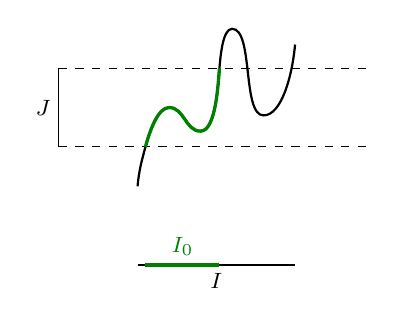
\begin{tikzpicture}
            \footnotesize
            \draw (1,0) -- node[below]{$I$} ++(2,0);
            \draw (0,1.5) -- node[left]{$J$} ++(0,1);
            \draw [dashed]
                (0,1.5) -- ++(4,0)
                (0,2.5) -- ++(4,0)
            ;
            \draw [green!50!black,very thick] (1.1,0) -- node[above]{$I_0$} (2.04,0);
    
            \draw [thick] (1,1)
                to [out=85,in=-105] (1.1,1.5)
                to [out=75,in=180,in looseness=0.6] (1.4,2)
                to [out=0,in=180] (1.8,1.7)
                to [out=0,in=-95,looseness=0.6] (2.04,2.5)
                to [out=85,in=180,looseness=0.6] (2.2,3)
                to [out=0,in=180,looseness=0.6] (2.6,1.9)
                to [out=0,in=-95,out looseness=0.6] (3,2.8)
            ;
            \draw [green!50!black,very thick] (1.1,1.5)
                to [out=75,in=180,in looseness=0.6] (1.4,2)
                to [out=0,in=180] (1.8,1.7)
                to [out=0,in=-95,looseness=0.6] (2.04,2.5)
            ;
        \end{tikzpicture}
        \caption{Loop mapping.}
        \label{fig:loopMapping}
    \end{figure}
    \begin{itemize}
        \item Isn't this obvious? No -- there's an issue, namely that $f(J_i)\not\subset J_{i+1}$. We can solve this though by noting that if $I\to J$, then there exists some subinterval $I_0\subset I$ such that $f(I_0)\subset J$ and $I_0\to J$ (i.e., $f(I_0)=J$).
        \item You can use this idea to pull a $J_i'$ out of each $J_i$ for which set equality holds.
        \item Then by the previous lemma, there exists a fixed point $p$ of $f^n$ in $J_0'$. Then $f(p)\in J_1'\subset J_1,\dots,f^{n-1}(p)\in J_{n-1}'\subset J_{n-1}$.
    \end{itemize}
    \item Notation.
    \begin{itemize}
        \item In the case of Lemma 3, we say that $p$ is \textbf{following} the cycle $J_0\to\cdots\to J_{n-1}\to J_0\to\cdots$.
        \item We call $J_0\to\cdots\to J_{n-1}\to J_0\to\cdots$ \textbf{elementary} if it is only followed by points of period $n$.
    \end{itemize}
    \item Lemma: Let $q$ have period $m$ and let $\mathcal{O}=\{q,f(q),\dots,f^{m-1}(q)\}$. Let $J_0\to\cdots\to J_{n-1}\to J_0\to\cdots$ and suppose
    \begin{enumerate}[label={(\roman*)}]
        \item all endpoints of the $J_i$ are in $\mathcal{O}$;
        \item the loop is not followed by any point in $\mathcal{O}$;
        \item The interior of $J_0$, $\text{int}\,(J_0)$ is disjoint from the other $J_i$.
    \end{enumerate}
    Then the loop is elementary, and so $f$ has a period $n$ point.
    \begin{itemize}
        \item Suppose $p$ follows the loop.
        \item Then by (i) and (ii), $p$ is not an endpoint of $J_0$, so if $f^i(p)=p\in J_0$ for $i<n$, then $\text{int}\,(J_0)\cap J_i$, contradicting (iii).
    \end{itemize}
\end{itemize}



\section{Chapter 9: Functions of Several Variables}
\emph{From \textcite{bib:Rudin}.}
\begin{itemize}
    \item \marginnote{2/15:}Defines a vector space by the closure of its elements under addition and scalar multiplication.
    \item Defines a linear combination, span, independence and dependence, dimension, basis, coordinates, and the standard basis.
    \item Theorem 9.2: If $X$ is spanned by $r$ vectors, $\dim X\leq r$.
    \item Corollary: $\dim\R^n=n$.
    \item Theorem 9.3: Let $X$ a vector space with $\dim X=n$.
    \begin{enumerate}[label={(\alph*)}]
        \item $E\subset X$ containing $n$ vectors spans $X$ iff $E$ is independent.
        \item $X$ has a basis, and every basis contains $n$ vectors.
        \item If $1\leq r\leq n$ and $\{\vec{y}_1,\dots,\vec{y}_r\}$ is independent in $X$, then $X$ has a basis containing $\{\vec{y}_1,\dots,\vec{y}_r\}$.
    \end{enumerate}
    \item Defines linear transformation, linear operator.
    \item Notes that $A\bm{0}=\bm{0}$ if $A$ is a linear transformation, and that $A$ is completely determined by its action on any basis.
    \item \textbf{Invertible} (linear operator): A linear operator $A$ that is one-to-one and onto.
    \item Theorem 9.5: $A$ a linear operator on $X$ finite-dimensional is one-to-one iff it is onto.
    \item Defines $L(X,Y)$, $L(X)$, the product $BA$ of two linear transformations, and the supremum norm of a linear transformation.
    \item Theorem 9.7:
    \begin{enumerate}[label={(\alph*)}]
        \item $A\in L(\R^n,\R^m)$ implies $\norm{A}<\infty$ and $A:\R^n\to\R^m$ uniformly continuous.
        \item $A,B\in L(\R^n,\R^m)$ and $c\in\C$ implies
        \begin{align*}
            \norm{A+B} &\leq \norm{A}+\norm{B}&
            \norm{cA} &= |c|\norm{A}
        \end{align*}
        Defining $d(A,B)=\norm{A-B}$ makes $L(\R^n,\R^m)$ a metric space.
        \item $A\in L(\R^n,\R^m)$ and $B\in L(\R^m,\R^k)$ implies
        \begin{equation*}
            \norm{BA} \leq \norm{B}\norm{A}
        \end{equation*}
    \end{enumerate}
    \item Theorem 9.8: Let $\Omega$ be the set of all invertible linear operators on $\R^n$.
    \begin{enumerate}[label={(\alph*)}]
        \item $A\in\Omega$, $B\in L(\R^n)$, and $\norm{B-A}\cdot\norm{A^{-1}}<1$ implies $B\in\Omega$.
        \begin{proof}
            Let $\norm{A^{-1}}=1/\alpha$, and let $\norm{B-A}=\beta$. Then
            \begin{align*}
                \norm{B-A}\cdot\norm{A^{-1}} &< 1\\
                \beta\cdot\frac{1}{\alpha} &< 1\\
                \beta &< \alpha
            \end{align*}
            To prove that $B\in\Omega$, the definition of invertibility and Theorem 9.5 tell us that it will suffice to show that $B$ is 1-1. To do so, it will suffice to show that $B\vec{x}=\bm{0}$ iff $\vec{x}=\bm{0}$. Let's begin. Let $\vec{x}\in\R^n$ be arbitrary. Then
            \begin{align*}
                \alpha|\vec{x}| &= \alpha|A^{-1}A\vec{x}|
                    \leq \alpha\norm{A^{-1}}\cdot|Ax|
                    = |A\vec{x}|
                    \leq |(A-B)\vec{x}|+|B\vec{x}|
                    \leq \beta|\vec{x}|+|B\vec{x}|\\
                (\alpha-\beta)|\vec{x}| &\leq |B\vec{x}|
            \end{align*}
            It follows that if $\vec{x}\neq\bm{0}$, then $|B\vec{x}|>0$. This combined with the fact that $B\bm{0}=\bm{0}$ implies the desired result.
        \end{proof}
        \item $\Omega$ is open in $L(\R^n)$ and $A\mapsto A^{-1}$ is continuous on $\Omega$.
        \begin{proof}
            To prove that $\Omega$ is open in $L(\R^n)$, it will suffice to show that for all $A\in\Omega$, there exists $N_r(A)$ such that if $\norm{B-A}<r$, then $B\in\Omega$. Let's begin. Let $A\in\Omega$ be arbitrary. Choose $N_\alpha(A)$ to be our neighborhood, where $\alpha$ is defined as in part (a). Let $B\in L(\R^n)$ satisfy $\norm{B-A}<\alpha$. Then $\norm{B-A}\cdot\norm{A^{-1}}<1$, so $B\in\Omega$ by part (a), as desired.\par
            To prove that $A\mapsto A^{-1}$ is continuous, it will suffice to show that $\norm{B^{-1}-A^{-1}}\to 0$ as $B\to A$. First off, we have by part (a) and the substitution $\vec{x}=B^{-1}\vec{y}$ ($\vec{y}\in\R^n$) that
            \begin{align*}
                (\alpha-\beta)|B^{-1}\vec{y}| &\leq |BB^{-1}\vec{y}| = |\vec{y}|\\
                \left| B^{-1}\left( \frac{\vec{y}}{|\vec{y}|} \right) \right| &\leq (\alpha-\beta)^{-1}
            \end{align*}
            Thus, since $|B^{-1}\vec{u}|$ is bounded by $(\alpha-\beta)^{-1}$ for every unit vector $\vec{u}\in\R^n$, $\norm{B^{-1}}$ is bounded by $(\alpha-\beta)^{-1}$. This combined with the fact that
            \begin{align*}
                B^{-1}-A^{-1} &= B^{-1}I-IA^{-1}\\
                &= B^{-1}AA^{-1}-B^{-1}BA^{-1}\\
                &= B^{-1}(A-B)A^{-1}
            \end{align*}
            implies by Theorem 9.7c that
            \begin{equation*}
                \norm{B^{-1}-A^{-1}} \leq \norm{B^{-1}}\norm{A-B}\norm{A^{-1}}
                \leq (\alpha-\beta)^{-1}\cdot\beta\cdot\frac{1}{\alpha}
                = \frac{\beta}{\alpha(\alpha-\beta)}
            \end{equation*}
            Therefore, since $\beta\to 0$ as $B\to A$, the above inequality establishes the desired result.
        \end{proof}
    \end{enumerate}
    \item Note that the mapping $A\mapsto A^{-1}$ defined in Theorem 9.8b is a 1-1 mapping of $\Omega$ onto $\Omega$ and its own inverse.
    \item Defines matrices, column vectors, and matrix multiplication.
    \item From the Schwarz inequality, we can show that
    \begin{equation*}
        \norm{A} \leq \left( \sum_{i,j}a_{i,j}^2 \right)^{1/2}
    \end{equation*}
    \item "If $S$ is a metric space, if $a_{11},\dots,a_{mn}$ are real continuous functions on $S$, and if for each $p\in S$, $A_p$ is the linear transformation of $\R^n$ into $\R^m$ whose matrix has entries $a_{ij}(p)$, then the mapping $p\to A_p$ is a continuous mapping of $S$ into $L(\R^n,\R^m)$" \parencite[211]{bib:Rudin}.
    \item \textcite{bib:Rudin} spends some time motivating the definition of the total derivative. He also discusses the natural 1-1 correspondence between $\R^1$ and $L(\R^1)$.
    \item Defines differentiability in $\R^n$.
    \item Theorem 9.12: $A_1,A_2$ the derivative of $\mathbf{f}$ at $\vec{x}$ implies $A_1=A_2$.
    \item If $\mathbf{f}:E\to\R^m$ where $E\subset\R^n$, then $\mathbf{f}':E\to L(\R^n,\R^m)$.
    \item $\mathbf{f}$ differentiable implies $\mathbf{f}$ continuous.
    \item Example ($\mathbf{f}$ is linear):
    \begin{itemize}
        \item If $A\in L(\R^n,\R^m)$, then $A'(\vec{x})=A$ for all $\vec{x}\in\R^n$. Note that this means that $A':\R^n\to L(\R^n,\R^m)$, as expected.
    \end{itemize}
    \item Theorem 9.15 (Chain Rule): $E$ open in $\R^n$, $\mathbf{f}:E\to\R^m$ differentiable at $\vec{x}_0\in E$, $I\supset\mathbf{f}(E)$ open in $\R^m$, and $\mathbf{g}:I\to\R^k$ differentiable at $\mathbf{f}(\vec{x}_0)$ implies $\mathbf{F}:E\to\R^k$ defined by
    \begin{equation*}
        \mathbf{F}(\vec{x}) = \mathbf{g}(\mathbf{f}(\vec{x}))
    \end{equation*}
    is differentiable at $\vec{x}_0$ with
    \begin{equation*}
        \mathbf{F}'(\vec{x}_0) = \mathbf{g}'(\mathbf{f}(\vec{x}_0))\mathbf{f}'(\vec{x}_0)\footnotemark
    \end{equation*}
    \footnotetext{Note that the right-hand side of this equation contains the product of two linear transformations.}
    \begin{proof}
        Largely symmetric to that of the one-dimensional chain rule in Chapter 5.
    \end{proof}
    \item \textbf{Components} (of $\mathbf{f}:\R^n\to\R^m$): The real functions $f_1,\dots,f_m$ defined by
    \begin{equation*}
        \mathbf{f}(\vec{x}) = \sum_{i=1}^mf_i(\vec{x})\vec{u}_i
    \end{equation*}
    for all $\vec{x}\in E$ or, equivalently, by $f_i(\vec{x})=f(\vec{x})\cdot\vec{u}_i$ ($1\leq i\leq m$), where $\vec{u}_1,\dots,\vec{u}_m$ is the standard basis of $\R^m$.
    \item Defines partial derivatives.
    \item Theorem 9.17: $E\subset\R^n$ open and $\mathbf{f}:E\to\R^m$ differentiable at $\vec{x}\in E$ imply the partial derivatives $(D_jf_i)(\vec{x})$ exist and
    \begin{equation*}
        \mathbf{f}'(\vec{x})\vec{e}_j = \sum_{i=1}^m(D_jf_i)(\vec{x})\vec{u}_i
    \end{equation*}
    for $1\leq j\leq n$.
    \item It follows that
    \begin{equation*}
        [\mathbf{f}'(\vec{x})] =
        \begin{bmatrix}
            (D_1f_1)(\vec{x}) & \cdots & (D_nf_1)(\vec{x})\\
            \vdots &  & \vdots\\
            (D_1f_m)(\vec{x}) & \cdots & (D_nf_m)(\vec{x})\\
        \end{bmatrix}
    \end{equation*}
    \item Discusses the gradient and the directional derivative.
    \item Theorem 9.19: $E\subset\R^n$ convex and open, $\mathbf{f}:E\to\R^m$ differentiable in $E$, and there exists $M$ such that
    \begin{equation*}
        \norm{\mathbf{f}'(\vec{x})} \leq M
    \end{equation*}
    for all $\vec{x}\in E$ implies
    \begin{equation*}
        |\mathbf{f}(\vec{b})-\mathbf{f}(\vec{a})| \leq M|\vec{b}-\vec{a}|
    \end{equation*}
    for all $\vec{a},\vec{b}\in E$.
    \item Corollary: If, in addition, $\mathbf{f}'(\vec{x})=\bm{0}$ for all $\vec{x}\in E$, then $\mathbf{f}$ is constant.
    \item \textbf{Continuously differentiable} (mapping $\mathbf{f}:E\to\R^m$): A function $\mathbf{f}:E\to\R^m$ such that $\mathbf{f}':E\to L(\R^n,\R^m)$ is continuous. \emph{Also known as} \textbf{$\bm{\pmb{\mathscr{C}}^1}$-mapping}. \emph{Denoted by} $\bm{\mathbf{f}\in\pmb{\mathscr{C}}^1(E)}$.
    \item Theorem 9.21: Let $E\subset\R^n$ open and $\mathbf{f}:E\to\R^m$. Then $\mathbf{f}\in\mathscr{C}^1(E)$ iff the partial derivatives $D_jf_i$ ($1\leq i\leq m$; $1\leq j\leq n$) exist and are continuous on $E$.
    \item \marginnote{2/20:}\textbf{Contraction} (of $X$ into $X$): A function $\varphi:X\to X$ for which there exists a number $c<1$ such that
    \begin{equation*}
        d(\varphi(x),\varphi(y)) \leq c\cdot d(x,y)
    \end{equation*}
    for all $x,y\in X$, where $X$ is a metric space with metric $d$.
    \item Theorem 9.23: $X$ a complete metric space and $\phi$ a contraction of $X$ into $X$ implies there exists a unique $x\in X$ such that $\varphi(x)=x$.
    \begin{proof}
        Let $x_0\in X$ be arbitrary. Define $\{x_n\}$ recursively by
        \begin{equation*}
            x_{n+1} = \phi(x_n)
        \end{equation*}
        for $n=0,1,2,\dots$. Let $c<1$ be the number corresponding to the contraction $\varphi$. Then for $n\geq 1$, we have
        \begin{equation*}
            d(x_{n+1},x_n) = d(\varphi(x_n),\varphi(x_{n-1})) \leq c\cdot d(x_n,x_{n-1})
        \end{equation*}
        or, for $n\geq 0$,
        \begin{equation*}
            d(x_{n+1},x_n) \leq c^nd(x_1,x_0)
        \end{equation*}
        by induction. Now to prove that $\{x_n\}$ is Cauchy, it will suffice to show that for all $\epsilon>0$, there exists $N$ such that $m\geq n\geq N$ implies $d(x_n,x_m)<\epsilon$. But since
        \begin{align*}
            d(x_n,x_m) &\leq \sum_{i=n+1}^md(x_i,x_{i-1})\\
            &\leq (c^n+c^{n+1}+\cdots+c^{m-1})d(x_1,x_0)\\
            &\leq [(1-c)^{-1}d(x_1,x_0)]c^n
        \end{align*}
        we can simply choose $N$ large enough that $[(1-c)^{-1}d(x_1,x_0)]c^N<\epsilon$. Thus, since $\{x_n\}$ is Cauchy and $X$ is complete, there exists $x\in X$ such that $\lim_{n\to\infty}x_n=x$. Therefore, since $\varphi$ is Lipschitz continuous, we have that
        \begin{equation*}
            \varphi(x) = \lim_{n\to\infty}\varphi(x_n)
            = \lim_{n\to\infty}x_{n+1}
            = x
        \end{equation*}
        as desired.\par
        Now suppose for the sake of contradiction that there exists $y\neq x$ such that $\varphi(y)=y$. Then since $\varphi$ is a contraction,
        \begin{equation*}
            d(y,x) = d(\varphi(y),\varphi(x)) \leq c\cdot d(y,x) < d(y,x)
        \end{equation*}
        a contradiction.
    \end{proof}
    \item Theorem 9.24 (Inverse Function Theorem): $E\subset\R^n$ open, $\mathbf{f}:E\to\R^n$ a $\mathscr{C}^1$-mapping, $\mathbf{f}'(\vec{a})$ invertible for some $\vec{a}\in E$, and $\vec{b}=\mathbf{f}(\vec{a})$ implies
    \begin{enumerate}[label={(\alph*)}]
        \item There exist $U,V\subset\R^n$ open with $\vec{a}\in U$, $\vec{b}\in V$ such that $\mathbf{f}$ is 1-1 on $U$ and $\mathbf{f}(U)=V$.
        \begin{proof}
            Let $A=\mathbf{f}'(\vec{a})$. Choose $\lambda$ such that
            \begin{equation*}
                2\lambda\norm{A^{-1}} = 1
            \end{equation*}
            Define\footnote{How do we motivate this definition?} for each $\vec{y}\in\R^n$ a function $\varphi$ by
            \begin{equation*}
                \varphi(\vec{x}) = \vec{x}+A^{-1}(\vec{y}-\mathbf{f}(\vec{x}))
            \end{equation*}
            for all $\vec{x}\in E$. (Note that a key property of $\varphi$ is that as defined, $\mathbf{f}(\vec{x})=\vec{y}$ iff $\vec{x}$ is a fixed point of $\vec{y}$.) Now since $\mathbf{f}\in\mathscr{C}^1$ and hence $\mathbf{f}'$ is continuous at $\vec{a}$, there exists an open ball $B_r(\vec{a})\subset E$ such that
            \begin{equation*}
                \norm{\mathbf{f}'(\vec{x})-A} < \lambda
            \end{equation*}
            for all $\vec{x}\in B_r(\vec{a})$. Let $U=B_r(\vec{a})$. Clearly it follows that $U$ is open. Thus, since each $\varphi'(\vec{x})=I-A^{-1}\mathbf{f}'(\vec{x})=A^{-1}(A-\mathbf{f}'(\vec{x}))$, we have that
            \begin{equation*}
                \norm{\varphi'(\vec{x})} \leq \norm{A^{-1}}\norm{A-\mathbf{f}'(\vec{x})}
                < \frac{1}{2\lambda}\cdot\lambda
                = \frac{1}{2}
            \end{equation*}
            Consequently, we have by Theorem 9.19 that for all $\vec{x}_1,\vec{x}_2\in U$,
            \begin{equation*}
                |\varphi(\vec{x}_1)-\varphi(\vec{x}_2)| \leq \frac{1}{2}|\vec{x}_1-\vec{x}_2|
            \end{equation*}
            Thus, by the uniqueness argument in the proof of Theorem 9.23, $\varphi$ has at most one fixed point in $U$, so $\mathbf{f}(\vec{x})=\vec{y}$ for at most one $\vec{x}\in U$. Therefore, $\mathbf{f}$ is 1-1 on $U$.\par
            Let $V=\mathbf{f}(U)$. To prove that $V$ is open, it will suffice to show that for all $\vec{y}_0\in V$, there exists an open subset of $V$ containing $\vec{y}_0$ such that. Let $\vec{y}_0\in V$ be arbitrary. By the definition of $V$ as the image of $U$ under $\mathbf{f}$, there exists $\vec{x}_0\in U$ such that $\mathbf{f}(\vec{x}_0)=\vec{y}_0$. As such, choose $B_r(\vec{x}_0)$ such that $\overline{B}\subset U$. Pick $\vec{y}$ satisfying $|\vec{y}-\vec{y}_0|<\lambda r$. Then
            \begin{equation*}
                |\varphi(\vec{x}_0)-\vec{x}_0| = |A^{-1}(\vec{y}-\vec{y}_0)|
                < \norm{A}\lambda r
                = \frac{r}{2}
            \end{equation*}
            so for all $\vec{x}\in\overline{B}$,
            \begin{align*}
                |\varphi(\vec{x})-\vec{x}_0| &\leq |\varphi(\vec{x})-\varphi(\vec{x}_0)|+|\varphi(\vec{x}_0)-\vec{x}_0|\\
                &< \frac{1}{2}|\vec{x}-\vec{x}_0|+\frac{r}{2}\\
                &\leq \frac{1}{2}\cdot r+\frac{r}{2}\\
                &= r
            \end{align*}
            Thus, $\varphi(\vec{x}_0)\in B$. Moreover, since $|\varphi(\vec{x}_1)-\varphi(\vec{x}_2)| \leq \frac{1}{2}|\vec{x}_1-\vec{x}_2|$ naturally holds for all $\vec{x}_1,\vec{x}_2\in\overline{B}\subset U$, we have that $\varphi$ is a contraction of $\overline{B}$ into $\overline{B}$. Additionally, since $\overline{B}\subset\R^n$ is closed, it is a complete metric space under the Euclidean metric. Thus, Theorem 9.23 implies that $\varphi$ has a fixed point $\vec{x}\in\overline{B}$. In particular, $\mathbf{f}(\vec{x})=\vec{y}$. Therefore, $\vec{y}\in f(\overline{B})\subset\mathbf{f}(U)=V$, as desired.
        \end{proof}
        \item If $\mathbf{g}$ is the inverse of $\mathbf{f}$ on $V$ [which exists by (a)], i.e.,
        \begin{equation*}
            \mathbf{g}(\mathbf{f}(\vec{x})) = \vec{x}
        \end{equation*}
        for all $\vec{x}\in U$, then $\mathbf{g}\in\mathscr{C}^1(V)$.
        \begin{proof}
            We first show that for all $\vec{y}\in V$, $\mathbf{g}'(\vec{y})=[\mathbf{f}'(\mathbf{g}(\vec{y}))]^{-1}$. Let $\vec{y}\in V$ be arbitrary, and choose $\vec{k}$ such that $(\vec{y}+\vec{k})\in V$. It follows by part (a) that there exist $\vec{x},\vec{x}+\vec{h}\in U$ such that $\vec{y}=\mathbf{f}(\vec{x})$ and $\vec{y}+\vec{k}=\mathbf{f}(\vec{x}+\vec{h})$. Thus,
            \begin{equation*}
                \varphi(\vec{x}+\vec{h})-\varphi(\vec{x}) = \vec{h}+A^{-1}[\mathbf{f}(\vec{x})-\mathbf{f}(\vec{x}+\vec{h})]
                = \vec{h}-A^{-1}\vec{k}
            \end{equation*}
            so
            \begin{equation*}
                |\vec{h}-A^{-1}\vec{k}| = |\varphi(\vec{x}+\vec{h})-\varphi(\vec{x})|
                \leq \frac{1}{2}|\vec{x}+\vec{h}-\vec{x}|
                = \frac{1}{2}|\vec{h}|
            \end{equation*}
            Consequently, $|A^{-1}\vec{k}|\geq\frac{1}{2}|\vec{h}|$, so
            \begin{equation*}
                |\vec{h}| \leq 2\norm{A^{-1}}|\vec{k}|
                = \frac{|\vec{k}|}{\lambda}
            \end{equation*}
            Additionally, we know that $\norm{\mathbf{f}'(\vec{x})-A}\norm{A^{-1}}=1/2<1$, so Theorem 9.8a implies that $\mathbf{f}'(\vec{x})$ is invertible with an inverse that we may call $T$. Thus, since
            \begin{align*}
                \mathbf{g}(\vec{y}+\vec{k})-\mathbf{g}(\vec{y})-T\vec{k} &= \vec{h}-T\vec{k}\\
                &= -T[(\vec{y}+\vec{k})-\vec{y}]+T\mathbf{f}'(\vec{x})\vec{h}\\
                &= -T[\mathbf{f}(\vec{x}+\vec{h})-\mathbf{f}(\vec{x})-\mathbf{f}'(\vec{x})\vec{h}]
            \end{align*}
            we have that
            \begin{equation*}
                \frac{|\mathbf{g}(\vec{y}+\vec{k})-\mathbf{g}(\vec{y})-T\vec{k}|}{|\vec{k}|} \leq \frac{\norm{T}|\mathbf{f}(\vec{x}+\vec{h})-\mathbf{f}(\vec{x})-\mathbf{f}'(\vec{x})\vec{h}|}{\lambda|\vec{h}|}
            \end{equation*}
            Consequently, $\vec{k}\to\bm{0}$ implies that $\vec{h}\to\bm{0}$, which implies that the right side of the above inequality goes to zero, which implies that the left side of the above inequality goes to zero. Thus, $\mathbf{g}'(\vec{y})=T$, so
            \begin{equation*}
                \mathbf{g}'(\vec{y}) = [\mathbf{f}'(\mathbf{g}(\vec{y}))]^{-1}
            \end{equation*}
            for all $\vec{y}\in V$, as desired.\par
            To prove that $\mathbf{g}'$ is continuous on $V$, Theorem 4.7 and the above equation tell us that it will suffice to show that $\mathbf{g}:V\to U$ is continuous, $\mathbf{f'}:U\to L(\R^n)$ is continuous, and $M\mapsto M^{-1}:L(\R^n)\to L(\R^n)$ is continuous. But we have the first condition since differentiability implies continuity and $\mathbf{g}$ is differentiable, we have the second condition since $\mathbf{f}\in\mathscr{C}^1$ by hypothesis, and we have the third condition by Theorem 9.8b, as desired.
        \end{proof}
    \end{enumerate}
    \item Theorem 9.25: $E\subset\R^n$ open, $\mathbf{f}::E\to\R^n$ a $\mathscr{C}^1$-mapping, and $\mathbf{f}'(\vec{x})$ invertible for all $\vec{x}\in E$ implies $\mathbf{f}(W)$ open in $\R^n$ for every open $W\subset E$.
    \begin{itemize}
        \item Note that the hypotheses of this theorem guarantee that $\mathbf{f}$ is locally 1-1 at each $\vec{x}\in E$, but it may not be 1-1 in $E$ under these conditions (see Exercise 9.17).
    \end{itemize}
\end{itemize}




\end{document}